\documentclass{report}
% \usepackage{arxiv}
\usepackage[utf8]{inputenc} % allow utf-8 input
\usepackage[T1]{fontenc}    % use 8-bit T1 fonts
\usepackage{hyperref}       % hyperlinks
\usepackage{url}            % simple URL typesetting
\usepackage{booktabs}       % professional-quality tables
\usepackage{amsfonts}       % blackboard math symbols
\usepackage{nicefrac}       % compact symbols for 1/2, etc.
\usepackage{microtype}      % microtypography
\usepackage{caption}
\usepackage{geometry,array,graphicx,float,caption}
\usepackage{subcaption}
% \usepackage{subfig}
\usepackage{graphicx} % for pdf, bitmapped graphics files
\usepackage{amsmath} % assumes amsmath package installed

\graphicspath{{./figures/}{./}}
\usepackage[normalem]{ulem}
\useunder{\uline}{\ul}{}

\title{Lyft 2019 Data Challenge - An analysis of drivers}

% \author{
%   Adam Li \\
%   Department of Applied Mathematics \& Statistics, \\
%   Department of Biomedical Engineering, \\
%   Johns Hopkins University, Baltimore, MD, 21218
%   \texttt{adam2392@gmail.com} 
% }
\begin{document}
% \maketitle

\textbf{Lyft 2019 Data Challenge - An analysis of drivers}

\section{Summary}
	% Background on Lyft
	Lyft has over 23 M users worldwide as of 2018, and claims 35\% of ride-sharing market as of May 2018. Drivers are an important aspect of Lyft's business model: they act as a revenue generator, as well as a platform customer because they give rides to passengers. We analyze driver and ride data over a three-month course of March 28th, 2016 to June 27th, 2016 with 194,081 total rides for 937 drivers. We present an analysis to estimate i) a driver-lifetime value (DLV) for a driver, ii) factors that affect this DLV, iii) average projected lifetime (APL) of a driver in weeks, iv) an investigation of driver behavior and finally v) recommendations based on these analyses.

	% DLV summary
	The amount of total revenue a driver brings to Lyft is generally controlled by two factors: the number of rides they give and the average revenue they collect per ride. We estimated the DLV by first estimating i) the number of rides per week on average that a driver gives, ii) the projected average lifetime of a driver in weeks, and iii) the average fare of a ride. We did not have any notion of cost per driver that Lyft incurs, so assumed a fixed cost per driver, we computed a DLV of \$6896.08 per driver and an APL of 26.44 weeks.

	% Driver behavior summary
	We identified two subsets of driver populations within the data based on the total \# rides given (with a cutoff at \$169). The DLV of this \textbf{3 month period} based on this was for Group A = \$72.87 $\pm$ \$1.66 and Group B = \$546.49 $\pm$ \$10.03. In addition to generating revenue, drivers are essential for maintaining Lyft's driver/rider economy, and so we want to have drivers that are reliant sources of revenue for Lyft and giving consistent rides to riders.

	\textbf{DLV = number rides per week X APL (in weeks) X average ride value = 138 X 26.44 X 1.89 = \$6896.08} 

\section{Results and Methods}
	Before any data analysis was done, we determined that in this dataset, all rides were completed by checking if everyone request was matched with an event ID for the end of the ride. However, there were 9262 ride with completed events without other data matching in the tables. This constituted of only ~4\% of total rides though, so we deemed this to be neglible. In addition, out of 937 drivers, there was no matching data for 100 of them (or NaN rows), which constitutes ~10\% of the drivers. We proceeded by analyzing the 837 drivers with 184819 rides as our complete dataset.

	\subsection{Methods}
		% High level code summary
		For the analysis stated, we used a combination of Python (Jupyter, Numpy, Pandas and Scipy) and Matlab (some extra plotting) hosted on: \href{https://github.com/adam2392/lyft_data_challenge}{link}. Instructions for reproducing in an Anaconda environment are left online. Three data tables were used: i) ride\_timestamps.csv, ii) ride\_ids.csv and iii) driver\_ids.csv.

		% Data used
		Before any data analysis was performed, the ride\_timestamps.csv file was analyzed to determine if there were any incomplete rides, and to compute time-of-day (four 6 hour bins starting at 12:00AM), day-of-week and month of the rides. Each ride was converted into the corresponding units of miles and minutes, and then used to compute the total fare, lyft revenue generated, fare due to primetime, fare due to mileage and fare due to time. These fare breakdowns give a holistic view of each ride, and allow us to determine the value for Lyft per ride, and the factors that affect the total fare in the ride (e.g. primetime (PT), mileage and time). We computed fares by writing a Python class for the Ride and Fare to compute for each respective ride. This could be easily extended to include tips, quality ratings and more complicated fares (e.g. Lyft Line). 

		% driver profiling
		We split drivers into profiles based on their first ride week (with respect to the start date of the dataset, March 28th, 2016). First ride week was defined as the week of the first ride after their onboarding date because we saw that a significant portion of drivers did not start in the week they were onboarded. This resulted in 8 sequential weeks with drivers that started driving. Week 8 only had data for 2 drivers starting, so we excluded those drivers from further analysis.

	\subsection{DLV}
	\subsubsection{Average Number Rides Per Week}

		To compute the average number of rides per week, we took the total number of rides per week, and normalized with respect to the total number of unique drivers that week. In figure \ref{fig:avg_rides_perweek}, we can see that when normalized, the number of normalized number rides per week is relatively distributed within the range of 138 $\pm$ 24 rides. This makes sense, since without normalizing, then the estimate of number of rides per week is heavily biased by the number of drivers out that week. When we multiply by the average number of unique drivers per week (496 $\pm$ 44), then we obtain an average of 68,475 rides per week total.

	\subsubsection{APL}

		To compute the APL for a driver, we took the average duration (in weeks) between a driver's first ride (after onboarding) and the driver's last ride. To compute this, we took the average cohort size for each week (i.e. the amount of drivers starting in that week), and tracked them over time of the dataset. The average cohort size was about 119 $\pm$ 16 drivers, excluding week 8. In figure \ref{fig:driver_cohort_over_time}, we look at the drivers stratified into their cohorts, defined by the week they start driving. It is clear that there is a downward trend in terms of the number of drivers within each cohort driving. So we found that on average, each cohort lost about 4.5 drivers per week after performing their first ride with Lyft. With an average cohort size of 119 drivers, then the average projected lifetime of a driver is 26.44 weeks. The downward trend makes sense because we expect drivers to be less likely to drive as time goes on. An average of 26.44 weeks is a little over 6 months, which seems like a reasonable period for an average Lyft driver to drive. Of course it is important to note, there are drivers that definitely drive significantly longer, and also significantly shorter within Lyft.

		\begin{figure}[!htb]
			\centering
			\begin{subfigure}[t]{0.49\textwidth}
			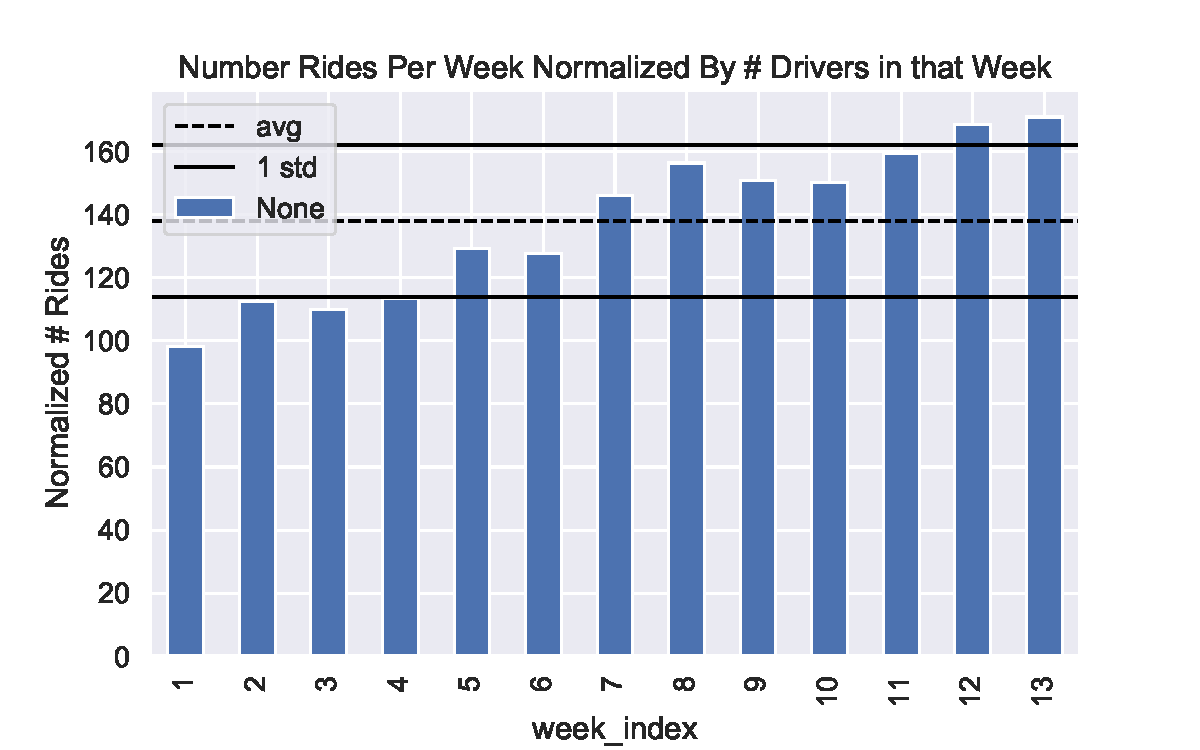
\includegraphics[width=\linewidth]{avg_number_rides_perweek.pdf}
			\caption{}
			\label{fig:avg_rides_perweek}
			\end{subfigure}
		% \end{figure} 
		% \begin{figure}[!htb]
			\centering
			\begin{subfigure}[t]{0.49\textwidth}
			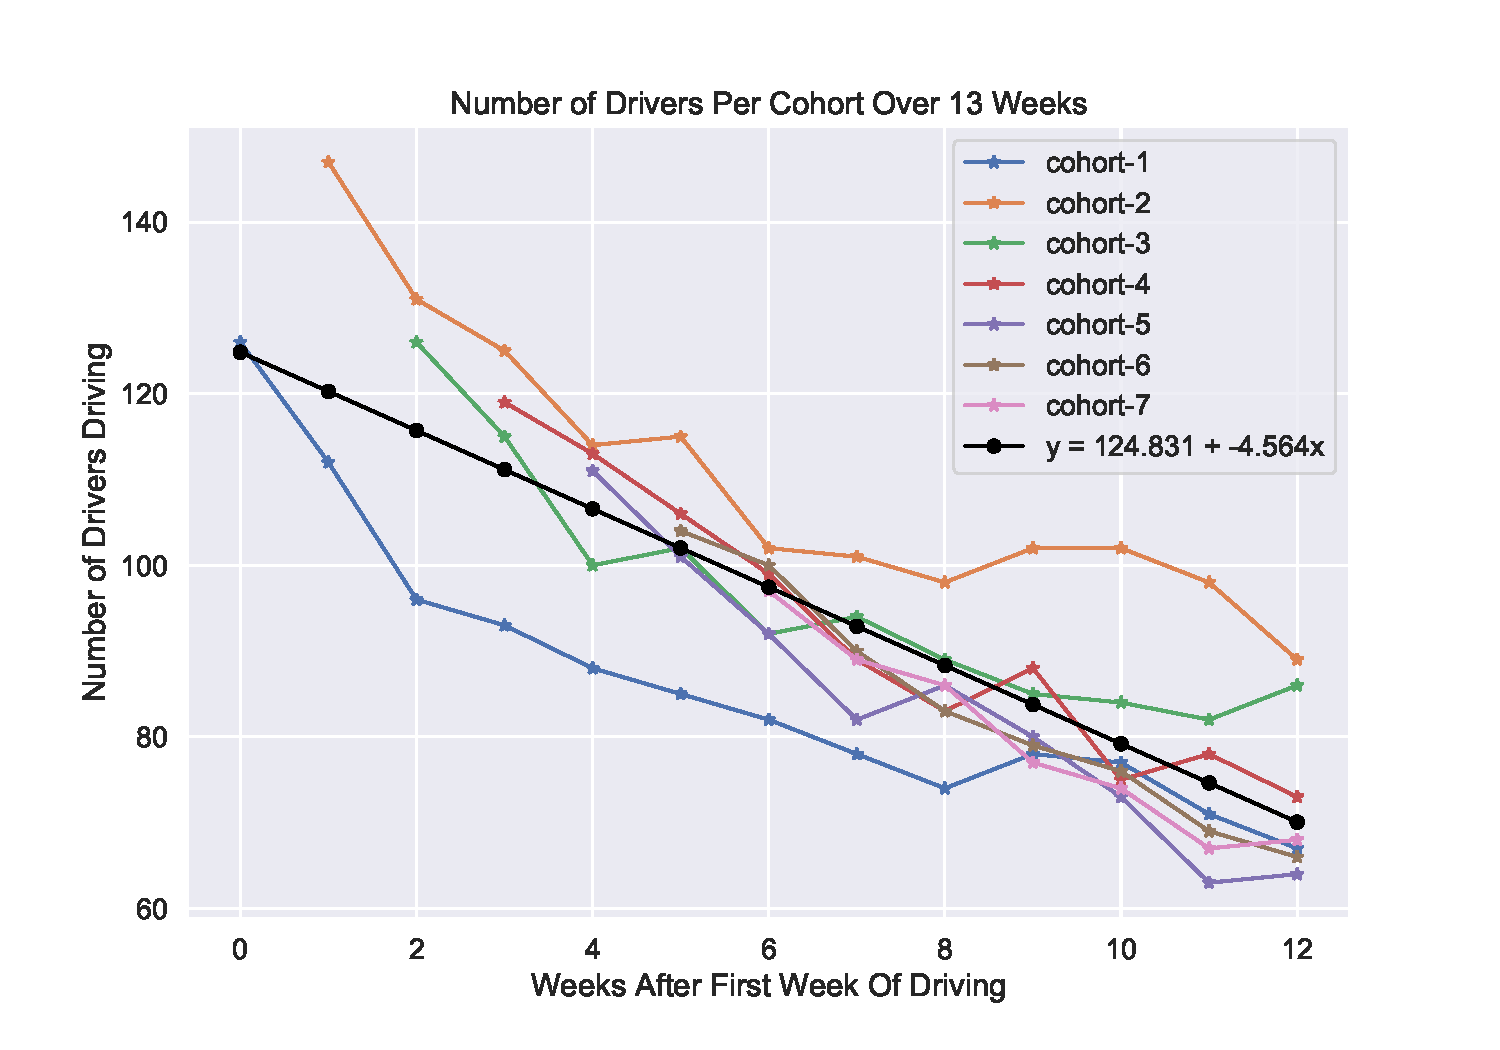
\includegraphics[width=\linewidth]{cohort_over_time.pdf}
			\caption{}
			\label{fig:driver_cohort_over_time}
			\end{subfigure}
			\caption{(a) Average number of rides per week normalized by the number of drivers. The average is 138 rides, with a standard deviation of 24 rides. and (b) Number of riders per cohort (defined by week they start driving) over time of the dataset. A linear regression line is fit with an $R^2$ value of 0.68 and a fit of 124.83 - 4.564x.}
		\end{figure} 

	\subsubsection{Average Ride Value}

		To compute the average ride value, we simply took the average fare total from all rides, and the standard deviation. This came out to an average fare of \$13.23 $\pm$ \$9.71 (from figure \ref{fig:driver_rev_distribution}c), which makes sense because most rides were relatively short rides. Note that it's important to note that Lyft's revenue is 20\% of this fare after subtracting the fees. With this in mind, the average ride value to Lyft would be \$1.89 (approximately 20\% of the fare value after taking off the fees). 

	\subsection{Factors for DLV: Revenue and Rides Generated For Lyft Per Driver}
		We first proceeded by computing DLV by first computing the average revenue generated by drivers for Lyft for all drivers in this dataset. We then proceeded by partitioning the driver populations into two populations, as in figure \ref{fig:driver_rev_distribution}, based on looking at the total rides given and total revenue generated. It is clear that there is a sub-population that is essentially giving very few rides, and also as a result generating less revenue. Specifically, we can see that at the 40th percentile out of the distribution of the number of rides given, we can categorize drivers into two subgroups: i) Group A (n=334 drivers): drivers with less then 83 rides and ii) Group B (n=507 drivers): drivers with more then 83 rides. We can think of these as "short-term" vs "long-term" drivers. Although rides and total revenue are different, the average fare per driver within each of these groups remain very similar: 13.56 $\pm$ 0.14 and 13.19 $\pm$ 0.06 for groups A and B respectively, suggesting that the differentiating factor is the term-length of driving between these driver populations. In group B, the APL for this subpopulation was estimated to be about 59 weeks, compared to the average over all the drivers of 26 weeks. This translates to a DLV of \$15,388.38 compared to our average of \$6896.08.

		\begin{figure}[!htb]
			\centering
			\begin{subfigure}[t]{0.32\textwidth}
				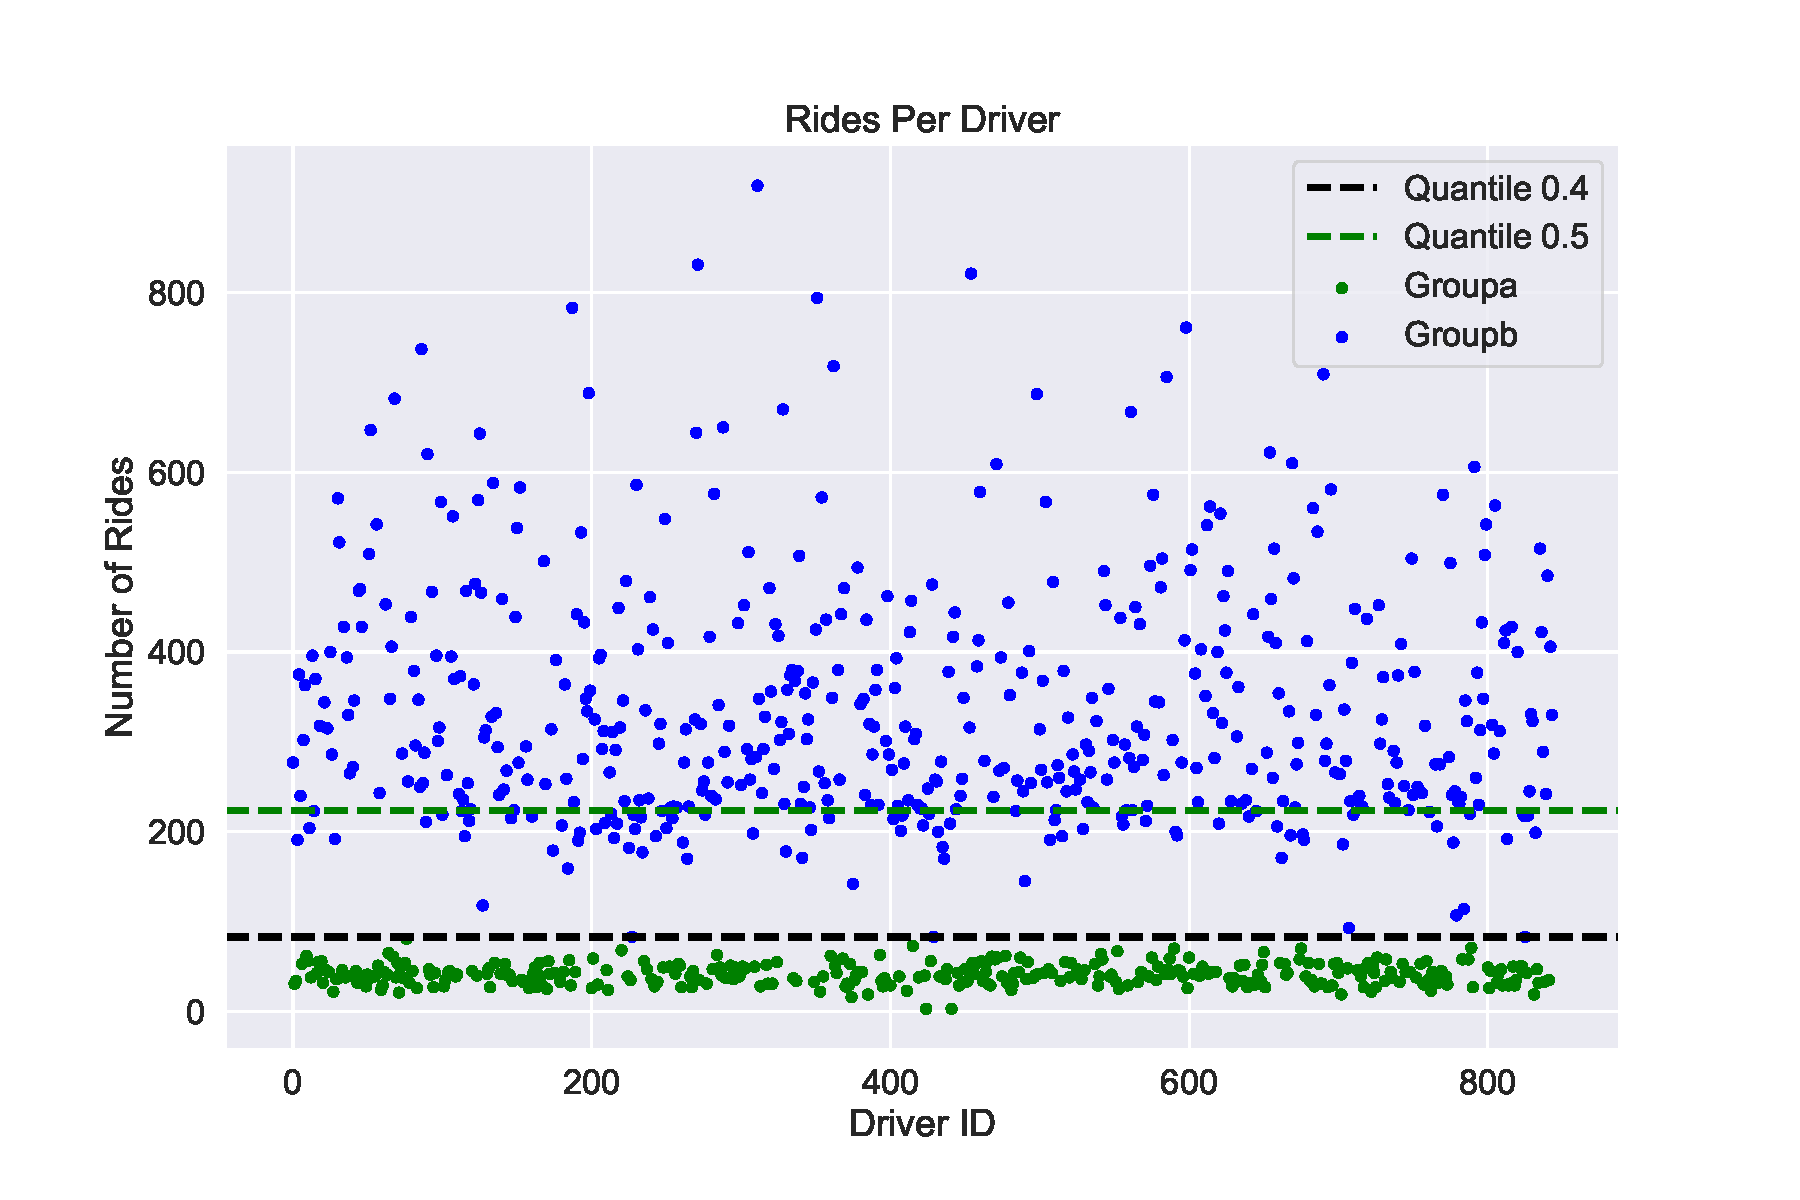
\includegraphics[width=\linewidth]{number_rides_per_driver.pdf}
				\caption{}
			\end{subfigure}
			\begin{subfigure}[t]{0.32\textwidth}
				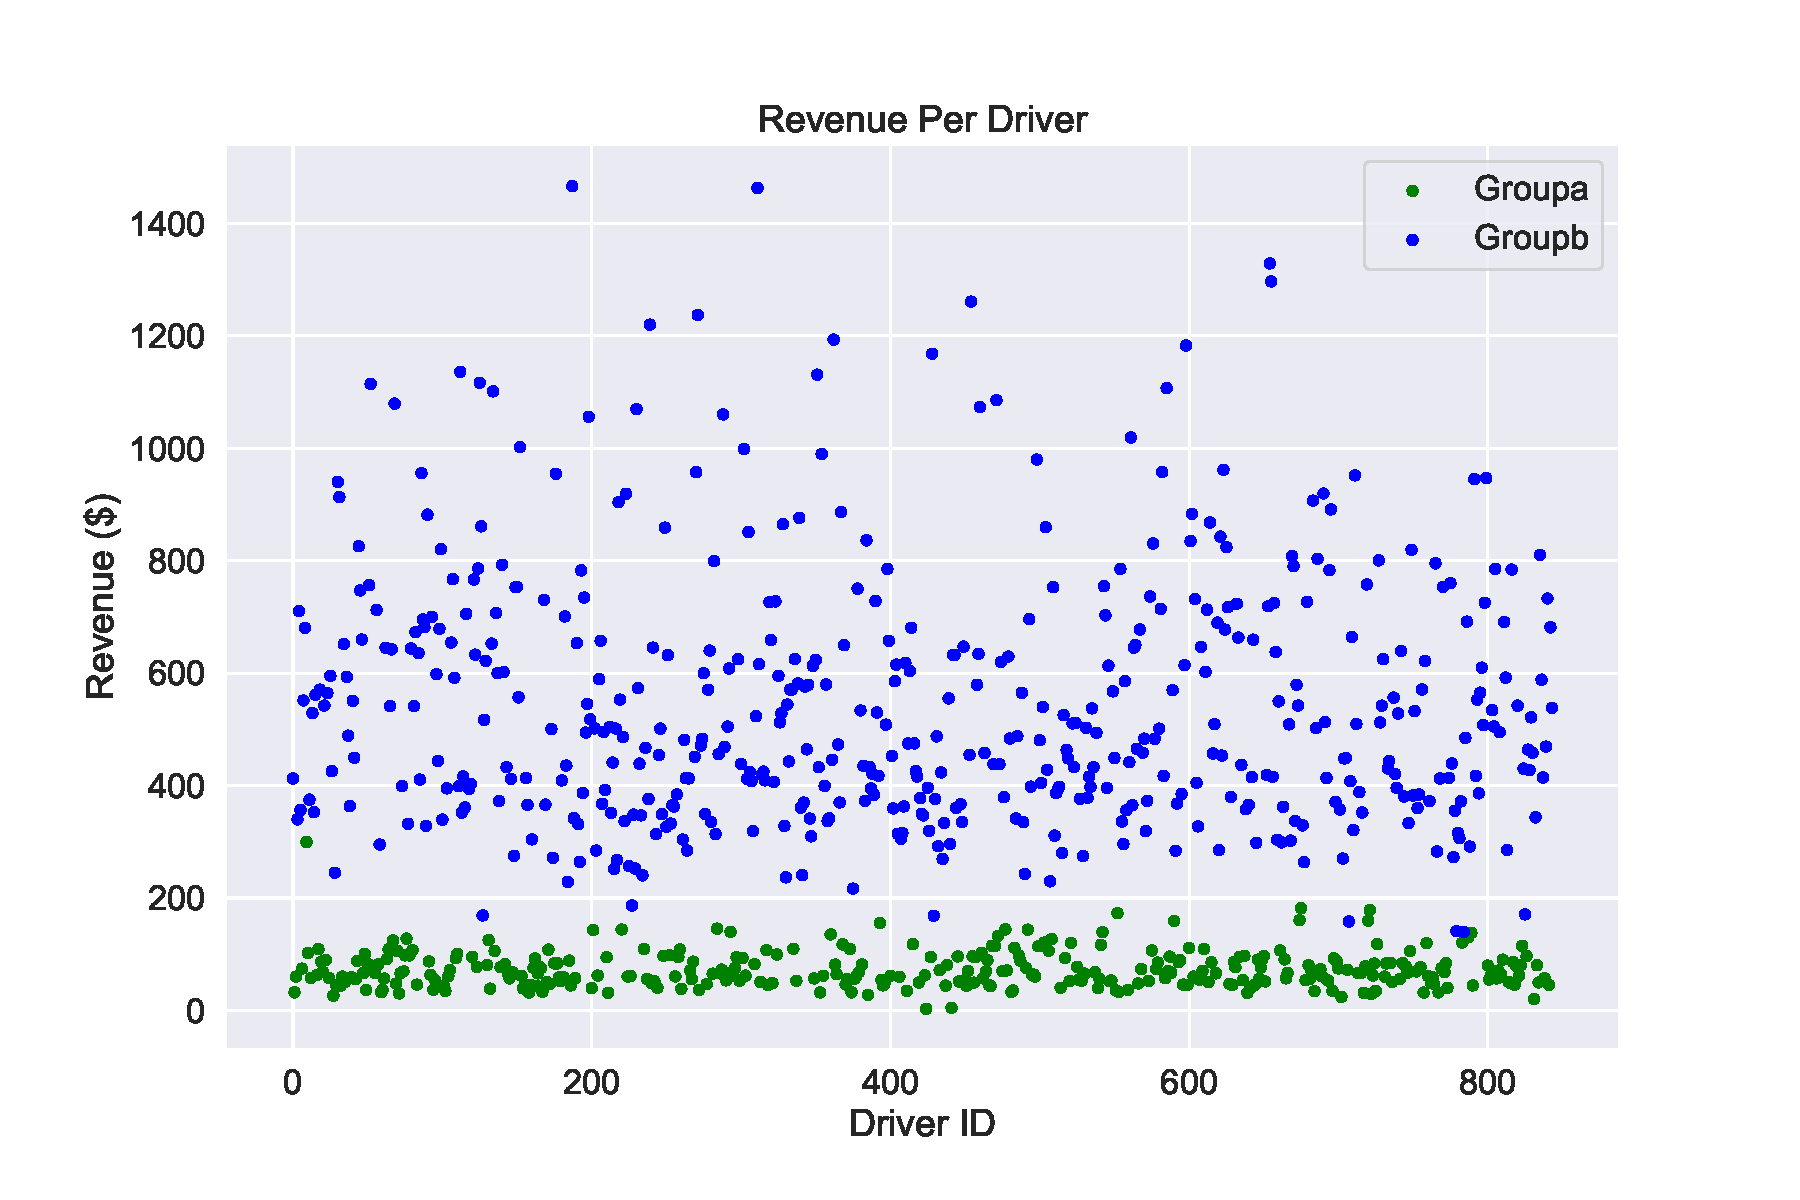
\includegraphics[width=\linewidth]{revenue_per_driver.pdf}
				\caption{}
			\end{subfigure}
			\begin{subfigure}[t]{0.32\textwidth}
				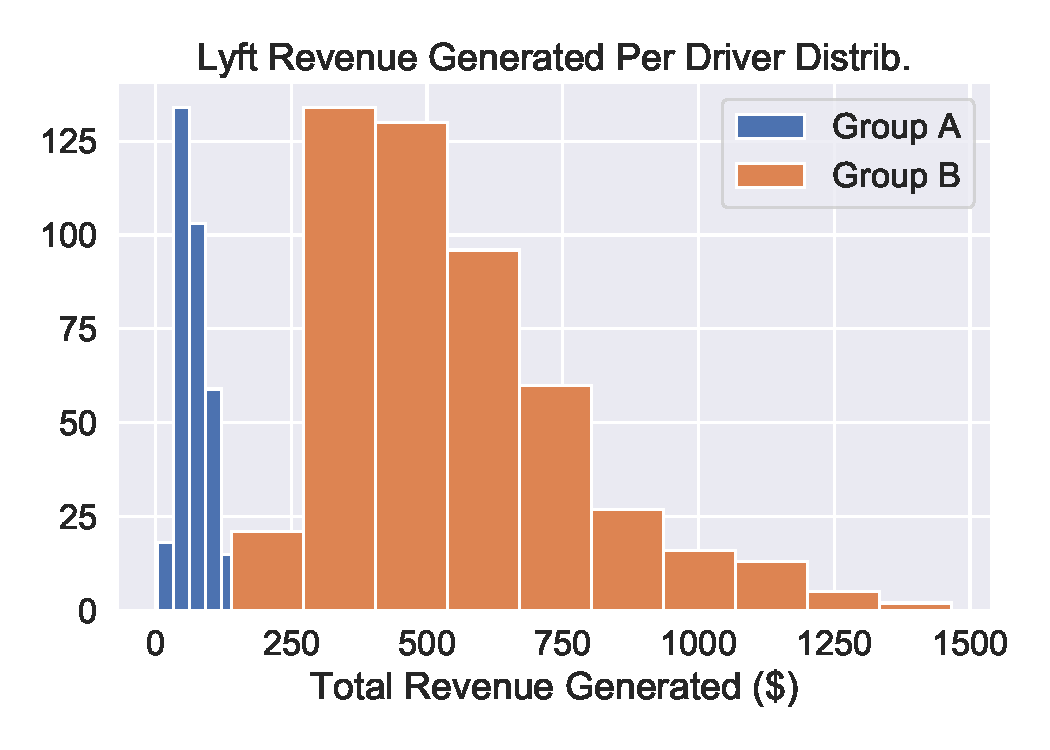
\includegraphics[width=\linewidth]{total_revenue_generated_perdriver_bimodal.pdf}
				\caption{}
			\end{subfigure}
			\caption{Total revenue generated per driver as a scatter plot (a) and total rides given per driver (b). The quantiles shown at 40th and 50th percentiles correspond to (83 rides/\$169), (224 rides/\$348) respectively. Total revenue generated for Lyft per driver with an average of \$356.82 $\pm$ \$10.02. The total revenue generated for lyft per driver now split based on the number of rides given into groups A and B (short term vs long term drivers), with an average of \$72.87 $\pm$ \$1.66 and \$546.49 $\pm$ \$10.03. The total revenue distribution for both groups are shown in (c).}
			\label{fig:driver_rev_distribution}
		\end{figure} 

	\subsection{Other Factors for DLV}

		We split these drivers into their respective groups: Group A and Group B (short and long term drivers). To investigate what factors affected the number of rides given, we looked at the rides given over the months, then over the days of the week, and then over the times of the day.

		\subsubsection{Time: Time-of-day, Day-of-week}
			First, we examined factors that determined average number of rides given per month, day-of-week and time-of-day. In figure \ref{fig:number_rides_time}, we see that number of rides given are concentrated during the late-evenings during the months May and June, and generally more on weekends, then weekdays (although not as strong of an effect). In figure \ref{fig:number_rides_pt}, we examined the presence of PT during the same periods. PT is correlated with rider demand, and we also saw the same trend, but with not as strong of a qualitative trend for the time of day. Based on both PT and number of rides given per driver, it seems that May and June are the busiest times with respect to riders, then the late evenings (6PM-12AM) and then generally weekends.

			% Effect of when it is? (month, day of week, time of day)
			\begin{figure}[!htb]
				\centering
				\begin{subfigure}[t]{0.32\textwidth}
					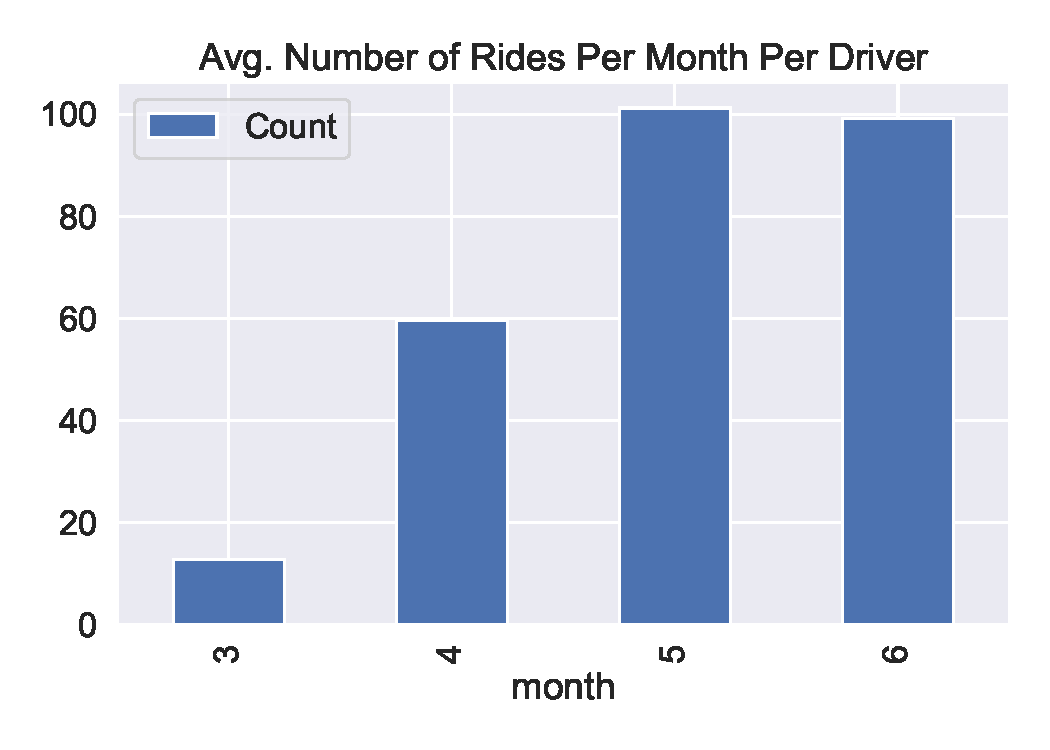
\includegraphics[width=\linewidth]{avg_number_rides_per_monthdriver.pdf}
					\caption{}
				\end{subfigure}
				\begin{subfigure}[t]{0.32\textwidth}
					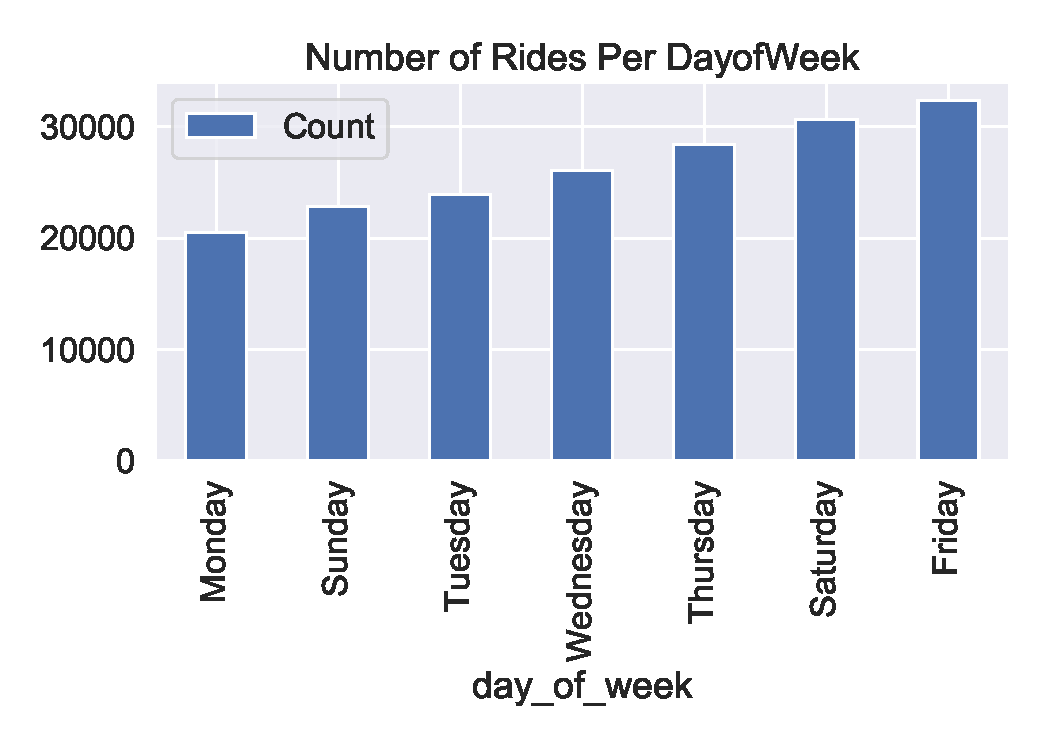
\includegraphics[width=\linewidth]{avg_number_rides_per_dayofweekdriver.pdf}
					\caption{}
				\end{subfigure}
				\begin{subfigure}[t]{0.32\textwidth}
					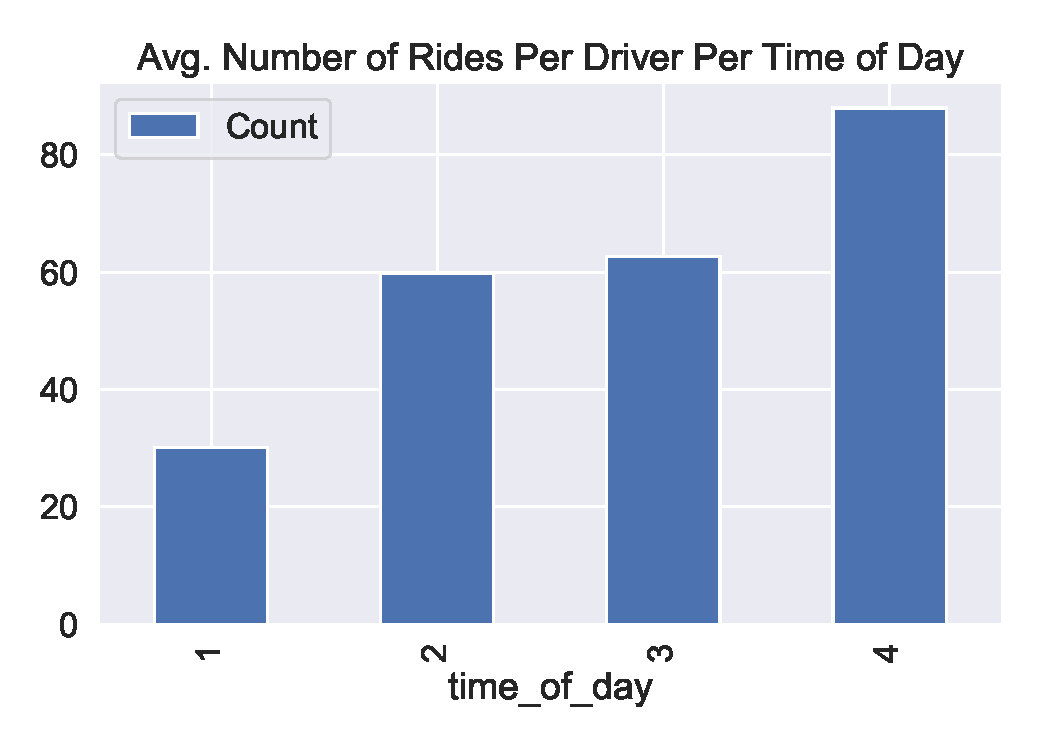
\includegraphics[width=\linewidth]{avg_number_rides_per_timeofdaydriver.pdf}
					\caption{}
				\end{subfigure}\\

				\centering
				\begin{subfigure}[t]{0.24\textwidth}
					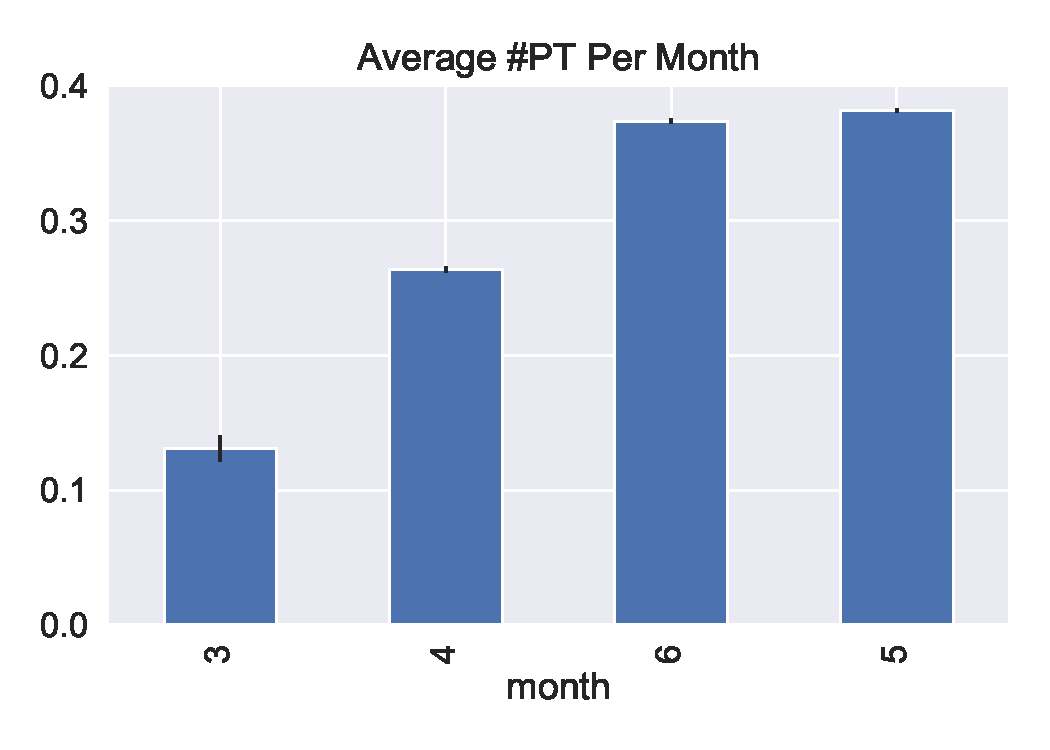
\includegraphics[width=\linewidth]{avg_number_pt_per_month.pdf}
					\caption{}
				\end{subfigure}
				\begin{subfigure}[t]{0.24\textwidth}
					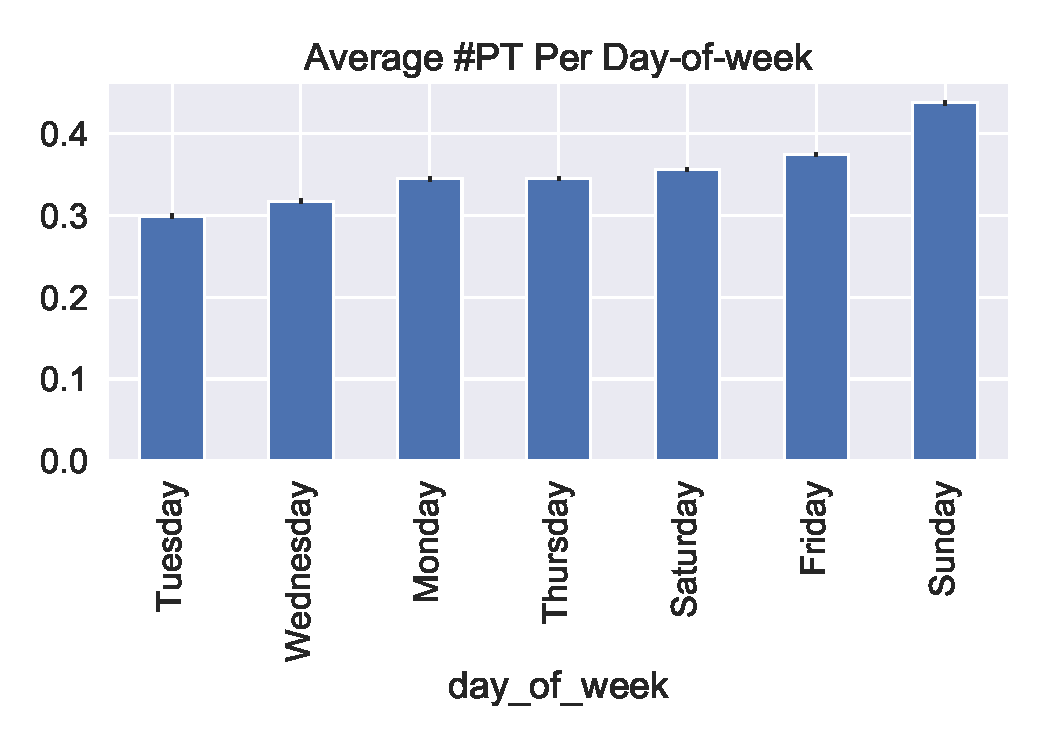
\includegraphics[width=\linewidth]{avg_number_pt_per_dayofweek.pdf}
					\caption{}
				\end{subfigure}
				\begin{subfigure}[t]{0.24\textwidth}
					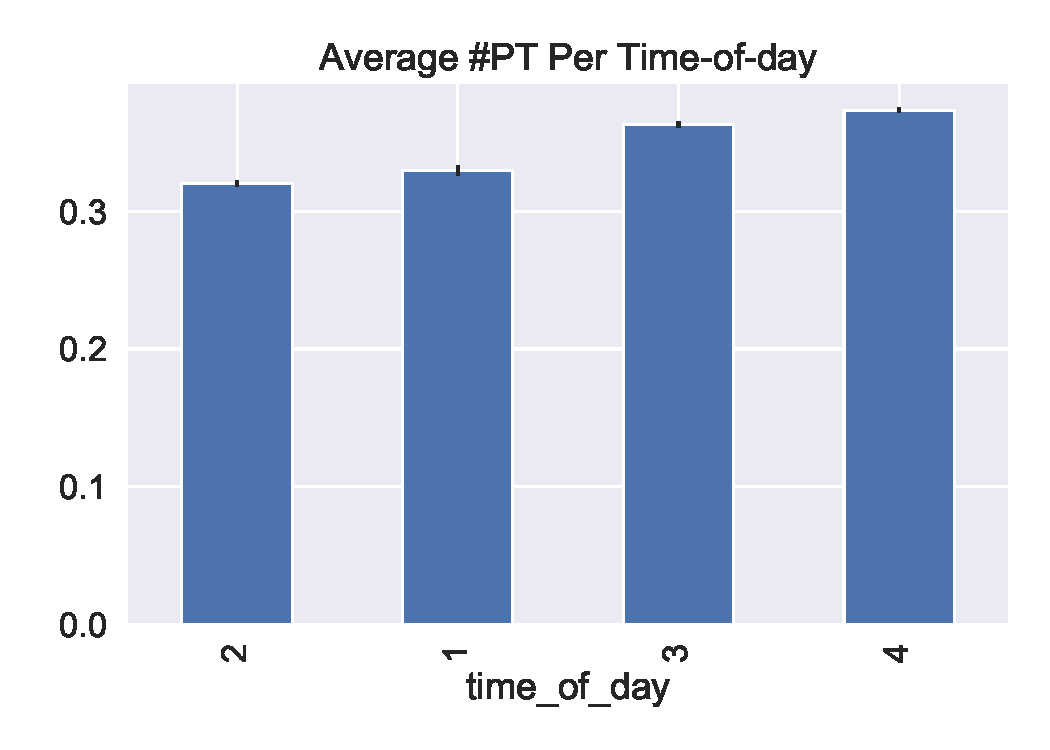
\includegraphics[width=\linewidth]{avg_number_pt_per_timeofday.pdf}
					\caption{}
				\end{subfigure}
				\begin{subfigure}[t]{0.24\textwidth}
					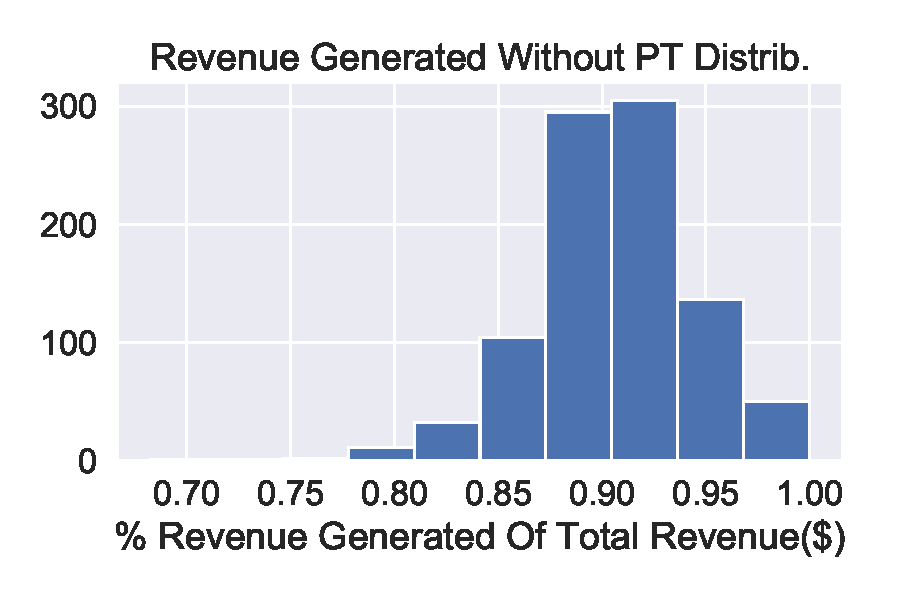
\includegraphics[width=\linewidth]{pre_pt_rev_percentage.pdf}
					\caption{}
				\end{subfigure}
				\caption{}
				\label{fig:number_rides_pt}

				\caption{For each driver, this was the average number of rides per time-factor, such as month (a), day-of-week (b) and time-of-day (c). There is an upward trend in the number of rides given in the months May and June, weekends (i.e. Friday and Saturday), and late-evenings. For details on how time-of-day is categorized, see Methods. For each driver, this was the average number of PT rides per time-factor, such as month (d), day-of-week (e) and time-of-day (f). There is an upward trend in the number of rides given in the months May and June, weekends (i.e. Friday and Saturday), and late-evenings. In (g), we see that most of the revenue from drivers did not come from PT.
				}
				\label{fig:number_rides_time}
			\end{figure}

		\subsubsection{Primetime}
			In addition, we looked at the effect of PT. In figure \ref{fig:number_rides_pt}, we see that PT is more prominent in May/June and weekends.

			% Effect of PT
			\begin{figure}[!htb]

			\end{figure} 

		\subsubsection{Ride Type: Mileage versus Time}
			We also looked at categorizations of rides based on their \% of fare due to mileage and time. We simply found that majority of rides were more due to milage, which makes sense since mileage is charged at \$1.15 per unit, versus \$0.22 per unit of time. 

\section{Recommendations}
	
	After analyzing this set of data, we determined an estimate of the APL of a driver as approximately 26.44 weeks and a corresponding DLV of \$6896.88. Along the way, we computed the average Lyft revenue from all the rides (of \$1.89), and the average number of rides per week (138), as well as factors that affect number of rides such as PT, mileage, time, time-of-day, day-of-week and month from the dataset. Since Group B population's DLV was at \$15,388 (more then double the overall average), we \textbf{first recommend} targeting this subpopulation of longer-term drivers. These drivers drive for significantly longer then Group A, give more rides, and as a result generate longer-term profits for Lyft. Lyft can implement a driver loyalty program that rewards longer-term driving (e.g. rewards for hitting 3, 6, or 12 months of driving) to incentivize driving longer term with Lyft. This has a number of beneficial effects: i) longer-term drivers are more efficient in navigating the app and ii) have more experience interacting with riders. 

	Another trend we saw late evenings (6PM-12AM), weekends (Friday/Saturdays) and May/June were periods of significantly more rides (in terms of both ride count and PT). Our \textbf{second recommendation} is to focus on i) recruiting drivers that can drive during these times and ii) getting drivers out during these times with targeted notifications. This can help combat problem of low driver-supply, and also help drivers earn more money. This in turn can help incentivize drivers to stay longer term with Lyft, and drive up their DLV.

	Some limitations that arise in analyzing the data was the amount of data points dropped in the rides, and driver groups. When we found drivers, or riders without their corresponding data points, then we dropped them, and this ended up being at most 9\% of the data. This does not seem like a major issue, unless these data points present a unique sub-population that is driving major revenues. Another limitation that was present in our dataset is the timeframe, and the locations for the dataset. Since we found interesting trends with respect to month, day-of-week and time-of-day, it would be necessary to validate these trends over a dataset that encompasses the entire year (ideally over multiple years). In addition, we can see if these trends hold across other cities.

\end{document}
